\section{Opinion Dynamics}

    Utilizzando i modelli di \textit{opinion dynamics} implementati nella libreria Python {\scshape NDlib}, si è voluto simulare le dinamiche di opinione sia sulla nostra rete indiretta di 16675 nodi, sia in uno scenario \textit{mean-field}, utilizzando un grafo completo ridimensionato a 3000 nodi, per ovviare all’elevato costo computazionale dell’operazione. 
    Ogni modello è stato testato con differenti configurazioni iniziali, mentre il numero di iterazioni è stato modulato in base all’andamento dell’opinione, nel tentativo di raggiungere - ove possibile - una situazione di convergenza, frammentazione o polarizzazione.\\ 
    
    \subsection{Modelli a opinione discreta}
    I modelli che utilizzano opinioni discrete - \textit{Voter}, \textit{Snayzd}, \textit{Majority Rule} e \textit{Q-Voter} - sono stati testati con quattro frazioni $f$ di nodi infetti iniziali differenti: 0.25, 0.5, 0.75 e 0.34, ovvero sulla frazione di “infetti” reale, calcolata come il rapporto tra il numero di nodi della rete con un valore di classificazione strettamente maggiore di 0 (utenti contrari al gesto di inginocchiarsi) e il numero totale di nodi della rete. Inoltre, per i modelli \textit{Majority Rule} e \textit{Q-Voter}, ogni frazione di nodi infetti è stata testata prendendo in considerazione un numero di vicini $q$ pari a 3, 5, 10 e 100 nodi. 
    Il \textit{Diffusion Trend plot} realizzato per le varie istanze è stato ottenuto modificando i colori proposti dalla libreria al fine di richiamare i colori utilizzati in questo lavoro (\ref{openq}) per indicare gli utenti contrari al gesto (rosso, gli ``infetti"), e quelli favorevoli al movimento (blu, i ``suscettibili"). 
    
    Nel \textit{Voter model}, la diffusione delle opinioni risulta essere molto lenta rispetto alle dimensioni della rete, probabilmente a causa di un tempo di simulazione ($10^2$-$10^3$ iterazioni) molto minore rispetto al tempo di convergenza del modello su questo tipo di topologie. Ciò avviene sia per quanto riguarda il \textit{mean field scenario} che per la rete reale, nella quale pare che il processo di diffusione rallenti ulteriormente: con uguale percentuale di infetti e suscettibili, infatti, nelle prime 500 iterazioni, la fluttuazione delle due frazioni nella rete reale avviene in un \textit{range} inferiore di circa un ordine di grandezza rispetto a quello osservato nella rete completa (quarta e terza cifra decimale). Ciò dipende, probabilmente, sia dalla minore connettività della rete reale, che implica dunque tempi di convergenza maggiori, sia dal suo carattere omofilo (par. \ref{subsection:echochamb}), che aumenta le probabilità dell'algoritmo di selezionare una coppia di nodi che posseggono già la stessa opinione.
    
    Il modello \textit{Sznajd}, al contrario, conduce la rete ad una convergenza dell’opinione sin dalle prime iterazioni nella rete completa, e in modo meno repentino ma altrettanto definito, nella rete generata dai dati raccolti, a prescindere dalla frazione di infetti iniziale.
    
    Per quanto riguarda i due modelli testati che permettono di considerare un numero di vicini a scelta, osservando il comportamento della rete con frazioni iniziali sbilanciate (0.25, 0.75, 0.34) si nota che, se nel \textit{Q-Voter} un numero di vicini basso (3, 5) sembra condurre l'opinione della rete alla convergenza, nel \textit{Majority Rule model}, la tendenza appare ribaltata: il tempo necessario alla convergenza, infatti, è tanto minore quanto più alto è il valore di $q$. 
    Partendo, invece, da un egual numero di nodi infetti e non infetti ($f = 0.5$) e scegliendo un insieme di vicini piccolo, entrambi i modelli generano una lunga serie di fluttuazioni dell'opinione; al contrario, quando $q$ = 10, se nel Majority Rule si raggiunge piena convergenza dell'opinione sin dalle primissime iterazioni, nella simulazione proposta dal \textit{Q-Voter}, condotta su 1000 iterazioni, lo stato della popolazione continua a fluttuare intorno allo 0.5. 
    
    
    \subsection{Modelli a opinione continua}
    
    \begin{figure*}[ht]
        \centering
        \begin{subfigure}{.4\textwidth}
            \caption{Random opinion - Complete Graph}
            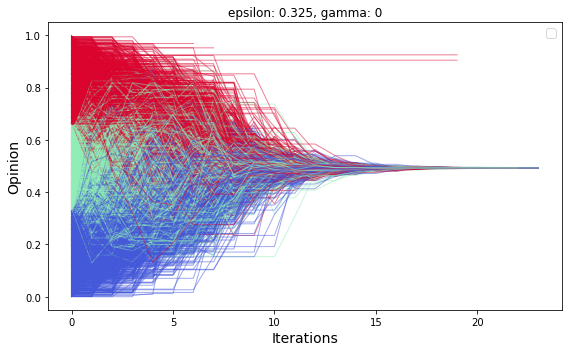
\includegraphics[scale=.25]{Opinion dynamics/random_complete_0_032.png}
            \label{fig:rdm_cmpl_0_032}
        \end{subfigure}
        \centering
        %\vspace{-3mm}
        \begin{subfigure}{.4\textwidth}
            \caption{Real opinion - Complete Graph}
            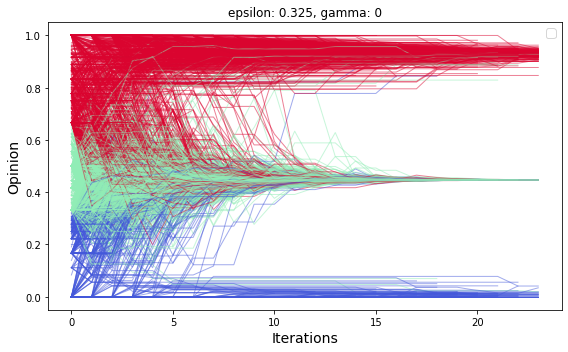
\includegraphics[scale=.25] {Opinion dynamics/real_complete_0_032.png}
            \label{fig:real_cmpl_0_032}
        \end{subfigure}
        \centering
        \begin{subfigure}{.4\textwidth}
            \caption{Random opinion - Crawled Graph}
            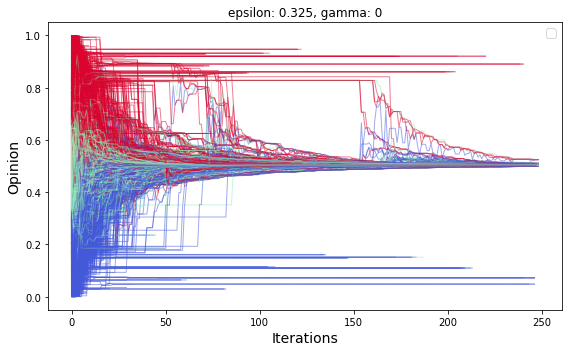
\includegraphics[scale=.25]{Opinion dynamics/random_crawled_0_032.png}
            \label{fig:rdm_crw_0_032}
        \end{subfigure}
        \centering
        %\vspace{-3mm}
        \begin{subfigure}{.4\textwidth}
            \caption{Real opinion - Crawled Graph}
            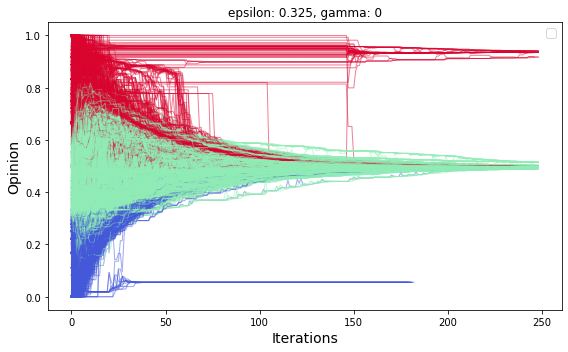
\includegraphics[scale=.25] {Opinion dynamics/real_crawled_0_032.png}
            \label{fig:real_crw_0_032}
        \end{subfigure}
        \caption{Simulazione dell'andamento dell'opinione con il modello Deffuant.}
        \label{fig:Deff}
    \end{figure*}
    
    Per quanto riguarda i modelli a opinione continua, ovvero il Deffuant con e senza bias, abbiamo testato due diversi valori di epsilon: 0.325 e il suo doppio, 0.65. Nel Modifies Deffuant Model, tali valori sono stati testati con quattro diversi valori di gamma (0.5, 1, 1.5, 5).
    Parallelamente, abbiamo ritenuto interessante applicare i modelli a opinione continua utilizzando come stato iniziale di ogni nodo non un valore random ma quello ottenuto dalle operazioni di classificazione dell'opinione del nodo $C_{u}$ (illustrate al par. \ref{subsection:class}), normalizzate tra 0 e 1, sostituendolo all’interno del file \texttt{AlgorithmicBiasModel}, alla variabile \texttt{self.status[node]} nella funzione \texttt{set\_initial\_status}. Anche in questo caso, abbiamo simulato l’andamento dell’opinione sia sulla rete reale, che su un grafo completo ottenuto estraendo randomicamente 3000 nodi dalla rete reale, collegandoli l’uno all’altro e assegnando a ciascuno di essi il proprio valore di classificazione.
    
    \subsubsection{Deffuant Model}
    Come ci si aspetta, il modello Deffuant ($\gamma$ = 0, nessun bias), quando applicato con un'alta \textit{open-mindness} ($\epsilon$ = 0.65), conduce l’opinione comune ad una situazione di convergenza, sia nella rete generata dai dati raccolti che nella rete completa, sebbene più lentamente quando le opinioni con cui vengono inizializzati i nodi sono reali. Con un'\textit{open-mindness} minore ($\epsilon$ = 0.325), invece, l'andamento delle opinioni è meno regolare. Infatti, se il modello conduce ad una situazione di convergenza, seppur non del tutto completa, nel \textit{complete graph} con opinioni random (fig. \ref{fig:rdm_cmpl_0_032}), quando ai suoi nodi vengono assegnati i rispettivi valori di classificazione, l'opinione si polarizza già dopo la quinta iterazione (fig. \ref{fig:real_cmpl_0_032}).
    Ancora diversa è la situazione della rete reale: in particolare, se si parte da opinioni random, la convergenza viene sì raggiunta nella maggior parte dei casi, ma in modo instabile e incompleto: non trascurabile è, infatti, la porzione di nodi le cui opinioni si frammentano, interrompendo le interazioni con gli altri nodi, sia tra i rossi che tra i blu (fig. \ref{fig:rdm_crw_0_032}). Partendo da opinioni reali, lo scenario è meno frammentato: i nodi tendono a creare due cluster principali - un'ampia frazione di nodi convergono verso l'opinione neutrale (0.5) e una parte polarizzata intorno all'opinione contraria ($\approx$ 0.80), oltre che ad un piccolo gruppo di nodi con opinione a favore ($\approx$ 0.05) che smette di interagire con la rete prima della duecentesima iterazione (fig. \ref{fig:real_crw_0_032}). Ciò può essere giustificato con la maggiore presenza nella rete di nodi con opinione $C_{u}>0.67$ (1 non normalizzato, in rosso) rispetto al numero di nodi con opinione $C_{u}<0.33$ (-1 non normalizzati, in blu). 
    
    \subsubsection{Modifies Deffuant Model}
    
      \begin{figure}
        \begin{subfigure}{.5\textwidth}
            \centering
            \caption{Random opinion}
            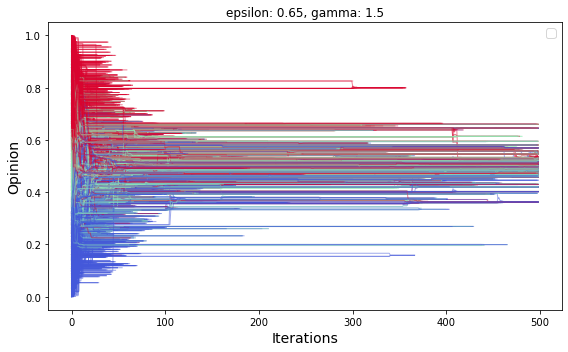
\includegraphics[scale=0.29]{Opinion dynamics/random_crawled_15_065.png}
            \label{fig:rdm_crw_15_065}
        \end{subfigure}
        \centering
        %\vspace{-3mm}
        \begin{subfigure}{.5\textwidth}
            \centering
            \caption{Real opinion}
            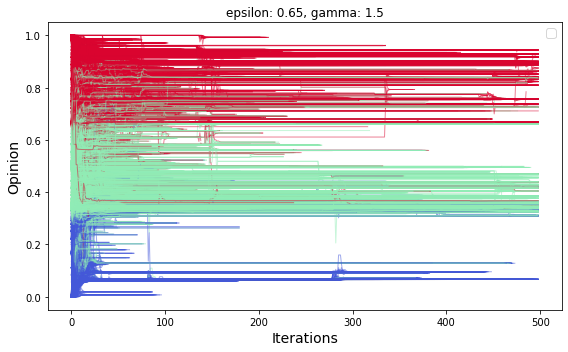
\includegraphics[scale=0.29] {Opinion dynamics/real_crawled_15_065.png}
            \label{fig:real_crw_15_065}
        \end{subfigure}
        \caption{Simulazione dell'andamento dell'opinione con il modello Modified Deffuant sulla rete reale.}
        \label{fig:ModDeff}
    \end{figure}
    
    Aumentando il bias ($\gamma$ $>$ 0), la rete, a prescindere dalla modalità con cui le opinioni iniziali vengono inizializzate, raggiunge la convergenza sempre più lentamente e in modo sempre più instabile e incompleto. Oltre $\gamma$ = 1, le opinioni dei nodi della rete si frammentano tanto più velocemente quanto più alto è il valore di $\gamma$ e basso il valore di $\epsilon$. Interessante, di nuovo, è il confronto tra il comportamento della rete inizializzata con opinioni random e con opinioni reali quando $\gamma$ è 1.5: se in entrambi i casi le opinioni si frammentano sin dalle prime iterazioni, è evidente come nel primo caso, la “discussione” persiste nella zona centrale del grafico, in cui sembrano confrontarsi nodi appartenenti a tutte e tre le “fazioni” (a favore, neutri e contrari), situazione ben diversa rispetto a quella che avviene quando ai nodi viene associato $C_{u}$, in cui lo scambio di opinioni si mantiene attivo principalmente intorno a due opinioni - contrari e neutri -, tanto più nettamente quanto più è alto il valore della \textit{open-mindedness} (fig. \ref{fig:ModDeff}).
    
    Per quanto riguarda il \textit{mean field scenario}, quando $\gamma$ è strettamente maggiore di 1, l’opinione si frammenta. Sotto questa soglia, invece, notiamo ancora una volta due andamenti differenti a seconda che i nodi vengano inizializzati con delle opinioni a valori reali o random: la popolazione della rete inizializzata in modo random converge ad un'unica opinione, tanto prima quanto minore è il valore del bias e maggiore il valore di $\epsilon$; al contrario, quando la rete viene inizializzata con i reali valori delle opinioni, il modello genera una polarizzazione dell’opinione generale, come del resto avveniva con il modello Deffuant (fig. \ref{fig:rdm_cmpl_0_032}). 
    
  